\documentclass{article}
\usepackage{graphicx} 
\usepackage{amsmath}
\usepackage{hyperref}
\usepackage[margin=1in]{geometry}
\usepackage{adjustbox}
\usepackage{import}
\date{}
\begin{document}
\thispagestyle{empty}
        \begin{figure}[h]
            \centering
            
\includegraphics[width=0.35\textwidth]{iitk_logo.jpg}
        \end{figure}

	\begin{center}
	\vspace{0.25cm}
	\LARGE
	\textbf{INDIAN INSTITUTE OF TECHNOLOGY KANPUR}
 
	\vspace{2.1cm}	
	\Large
\textbf{\huge Stock Market Analysis and Forecasting}
	\vspace{1.5cm}
	\normalsize	
	\\ \large Prepared By \\
	\vspace{.2cm}
	\begin{table}[h]
            \centering
            \resizebox{0.55\textwidth}{!}{
            \begin{tabular}{|c|c|}
                \hline
                \textbf{Roll Number} & \textbf{Group Member} \\
                \hline
                221312 & Dhairya Daga \\
                221327 & Kanchan Maan \\
                210954 & Shabadpreet Singh \\
                221416 & Shailza Sharma\\
                \hline
            \end{tabular}
            }
        \end{table}

	
	\vspace{1.3cm}
	\normalsize	
	   \large Under the supervision of  \\
	\vspace{.2cm}
	\large
	\textbf{\Large Prof. Amit Mitra \\ Dept. of Mathematics and Statistics } 	
 
	\vspace{3.5cm}
	\date{ 12 NOVEMBER 2023}
        {\textbf12 NOVEMBER 2023}
	\end{center}
	
\newpage
\tableofcontents
\newpage 
\section{Introduction}
Time Series analysis consists of methods used for analyzing the time series data so that we are able to get meaningful characteristics from the data that we had. We use time series forecasting in order to use a model so that we are able to predict future values which are based on the values which were previously observed. We can predict the trends present in financial markets or even electricity consumption, using time as an important factor.

The data used in our project is the stock market data of the Nifty-50 index (Reliance Industries) from the National Stock Exchange which has been taken over a period from the year 2000 to 2020.
VWAP means Volume Weighted Average Price which is the target variable in our case, that we are going to predict.
VWAP is a benchmark used by the traders that can give them the average price the stock would have traded throughout the month, which has been based on two important factors that are volume and price.


\textbf{About dataset :}
We have extracted the data from the official \href{https://www.nseindia.com}{National Stock Exchange} website.


\begin{figure}[h]
    \centering
    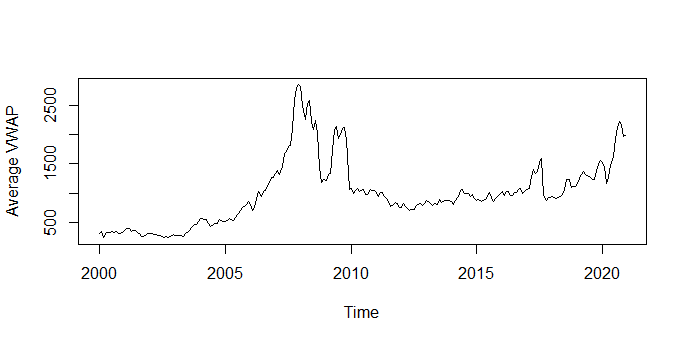
\includegraphics[width=0.9\textwidth]{Intro_plot_1.png}
    % Add a caption for the graph
    \caption{Visualizing Data}
    % Assign a label for referencing in the document
    \label{fig:Label1}
\end{figure}

\subsection{Mean and Variance Analysis}
\begin{figure}[h]
    \centering
    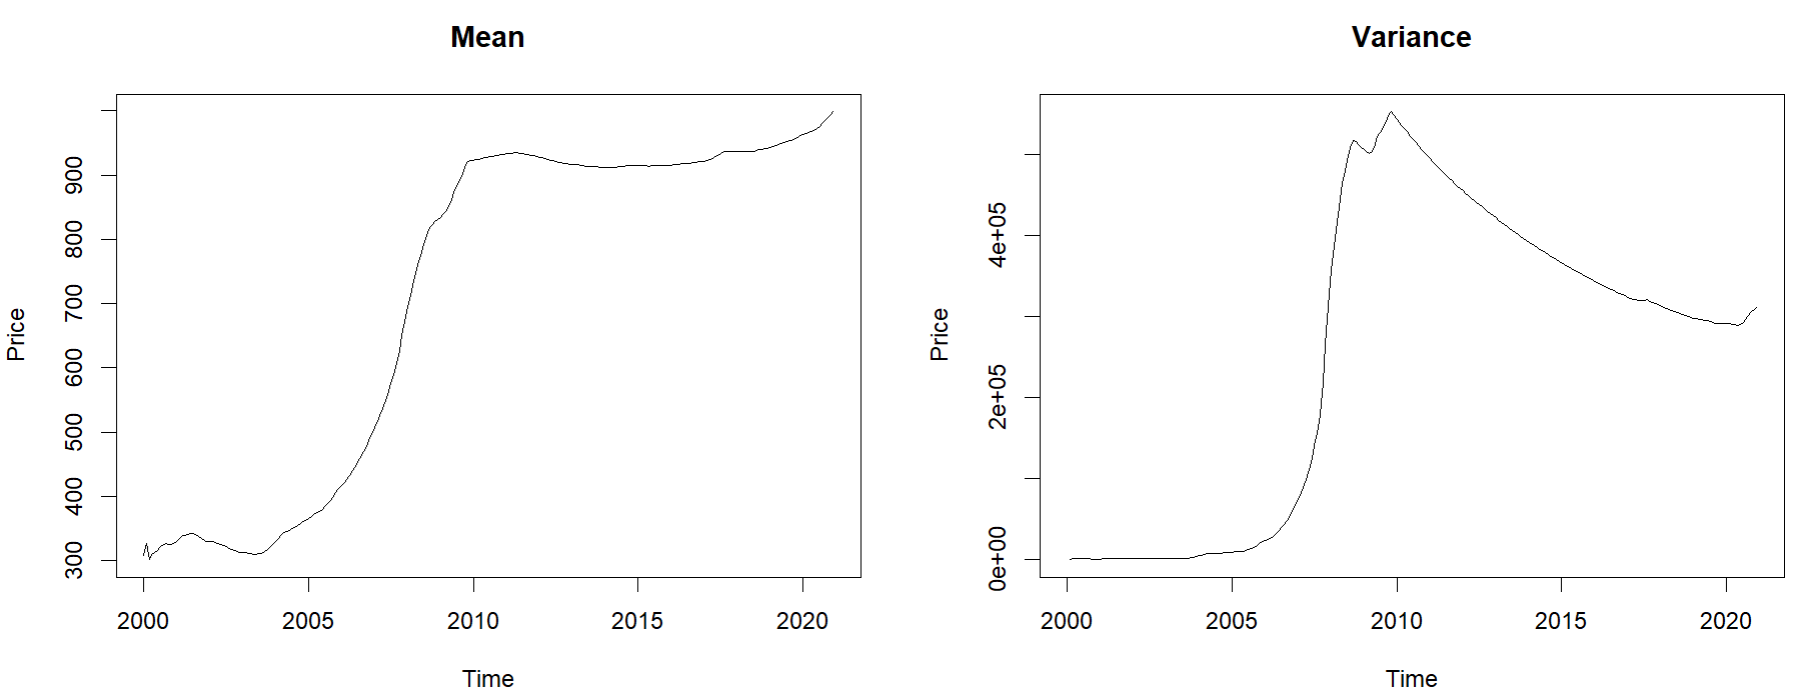
\includegraphics[width=0.9\textwidth]{MeanVarianceBefore.png}
    % Add a caption for the graph
    \caption{Mean and Variance of Original Series}
    % Assign a label for referencing in the document
    \label{fig:Label2}
\end{figure}

We see that the time series has a large mean and variance, so we instead work with the logarithmic time series.

\begin{figure}[h]
    \centering
    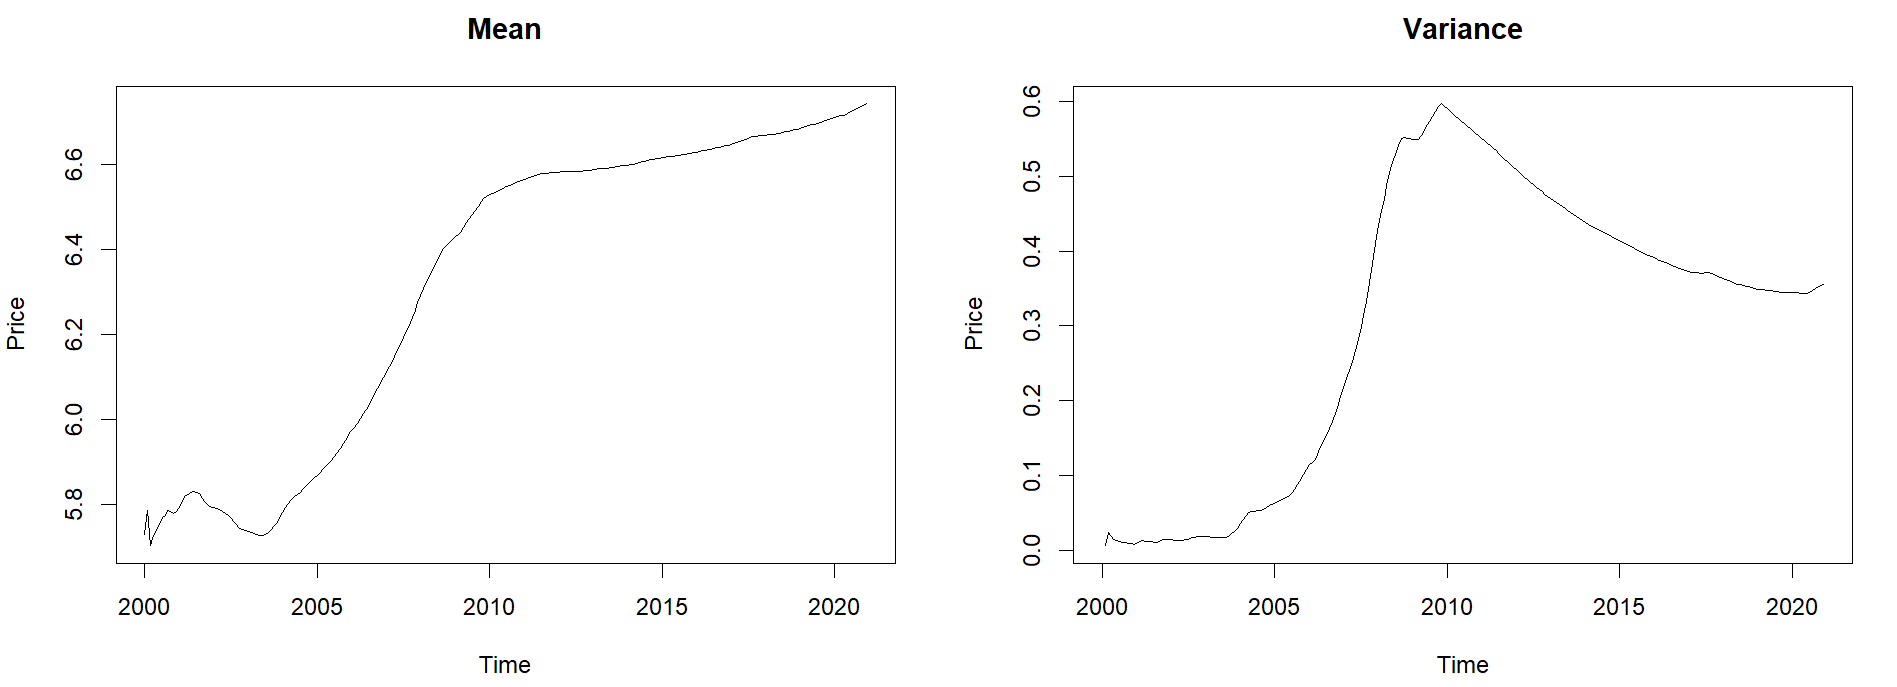
\includegraphics[width=0.9\textwidth]{MeanVarianceAfter.png}
    % Add a caption for the graph
    \caption{Mean and Variance of Logarithmic Series}
    % Assign a label for referencing in the document
    \label{fig:Label3}
\end{figure}

We now have significantly reduced the mean and variance, now we will continue with various tests.

\section{Randomness of the Data}
The first step in this process is to check the randomness of the data.

\begin{center}
    \textbf{Turning Point Test}.
    
    Null Hypothesis (\(H_0\)): The series is purely random.
    
    Alternative Hypothesis (\(H_1\)): The series is not random.
\end{center}

\( Y_i \) is a turning point if \( Y_i > Y_{i-1} \) and \( Y_i > Y_{i+1} \) or \( Y_i < Y_{i-1} \) and \( Y_i < Y_{i+1} \). 

\( T_i \) is defined as:
\[ 
T_i = 
\begin{cases}
    1 & \text{if } Y_i \text{ is a turning point} \\
    0 & \text{otherwise}
\end{cases}
\]

\[ T = \sum_{i=2}^{n-1} T_i. \]
\[ Z = \frac{T - E[T]}{\sqrt{V(T)}} \sim \mathcal{N}(0,1) \text{ under } H_0. \]

Given that \( E(T) = \frac{2(n-2)}{3} \) and \( V(T) = \frac{16n - 29}{90} \),

The test criterion is to reject \( H_0 \) at the \( \alpha \) level of significance (\textit{l.o.s.}) if \( \lvert \text{obs } Z \rvert > Z_{\alpha/2} \).

Given \( \lvert Z \rvert = \textbf{8.796} > 1.96 \) (\( Z_{0.025} \)), we reject our null hypothesis at the 5\% \textit{l.o.s.}.

Thus, our data is deemed not random, suggesting the presence of some trend in the model. The subsequent step involves exploring and identifying the specific trends within the dataset.

\section{Presence of Trend and Seasonality}

\subsection{Test the presence of Trend }
\textbf{Relative Ordering Test}
\begin{center}
      Null Hypothesis (\(H_0\)): No trend
    
    Alternative Hypothesis (\(H_1\)): Trend is present
\end{center}
R - Number of discordant pairs

If \(R > E(R)\), it indicates a falling trend. If \(R < E(R)\), it indicates a rising trend. Here, \(R\) is related to Kendall’s Tau (\(T\)), the rank correlation coefficient, given by \(T = 1 - \frac{4R}{n(n-1)}\).

Under \(H_0\), \(E(T) = 0\) and \(V(T) = \frac{2(2n+5)}{9n(n-1)}\).

The test statistic is \(Z = \frac{T - E(T)}{\sqrt{V(T)}} \sim \mathcal{N}(0,1)\).

The test criterion is to reject \(H_0\) if observed \(|Z| > Z_{\alpha/2}\) at the \(\alpha\) level of significance.

Given that \(R = 8524 \) and \(E(R) = 166.67\), there is a rising trend in our model. \(|Z| = 10.9> 1.96\) (\(Z_{0.025}\)), and hence we reject our null hypothesis.

We can conclude , there is \textbf{trend}.




\subsection{Trend Elimination}

The method used for trend elimination is Differencing of order 1 , and then we again check for the presence of trend. If trend is present we again use differencing and check for trend presence again, we repeat this method until the trend is removed completely.

\begin{figure}[h]
    \centering
    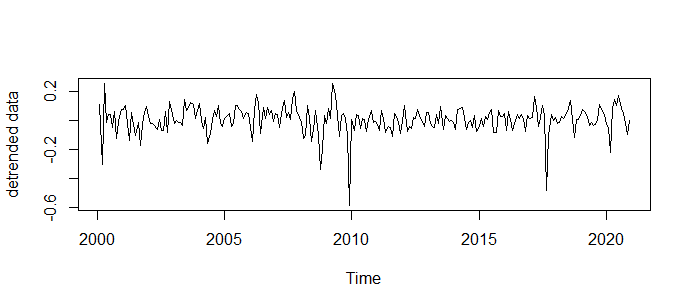
\includegraphics[width=0.9\textwidth]{Detrended_Data.png}
    % Add a caption for the graph
    \caption{Detrended Data}
    % Assign a label for referencing in the document
    \label{fig:Label4}
\end{figure}

\newpage
\subsection{Test the presence of Seasonality }
\textbf{Friedman's Non Parametric Test }

\begin{center}
    Null Hypothesis (\(H_0\)): No Seasonality
    
    Alternative Hypothesis (\(H_1\)): Seasonality is present
\end{center}

In the context of a specific month, the occurrence of higher ranks (ranking for that particular month and year) signifies seasonal peaks. On the other hand, if there is no inherent seasonality in the monthly data, the assigned ranks to the values should be distributed randomly. To establish a test statistic, our initial step involves calculating the month totals (\(M_i\)).

The test statistic \(X\) is given by the formula:

\[ X = 12 \sum_{i=1}^{r} \frac{(M_i - \frac{c(r+1)}{2})^2}{cr(r+1)} \]

where \(r\) represents the month and \(c\) is the year.

Under the null hypothesis, \(X\) follows a chi-squared distribution with \(r-1\) degrees of freedom (\(X \sim \chi^2(r-1)\)).

We reject the null hypothesis if the observed chi-square value (\(\chi^2_{\text{observed}}\)) is greater than the tabulated value (\(\chi^2_{r-1}\)). \\
In this case, with \(r = 19\) and \(c= 21\), the observed value of chi-square is (10.11), which is \textbf{smaller} than the tabulated value (19.67). 

Therefore, we fail to reject the null hypothesis and conclude that \textbf{seasonality may not be present.}




\section{Stationarity Check}
In time series analysis, a stationary time series is one whose mean, variance, and autocorrelation,stay constant over time.A time series \(\{X_t\}\) is stationary if it has:

1. \textbf{Constant Mean:} The mean of the series (\(\mu\)) is constant for all time points, i.e., \(E(X_t) = \mu\) for all \(t\).

2. \textbf{Constant Variance:} The variance of the series (\(\sigma^2\)) is constant for all time points, i.e., \(\text{Var}(X_t) = \sigma^2\) for all \(t\).

3. \textbf{Constant Autocorrelation:} The autocorrelation between observations at different time points (\(\rho_k\)) is constant for all lags \(k\), i.e., \(\text{Corr}(X_t, X_{t+k}) = \rho_k\) is constant for all \(t\) and \(k\).

Stationarity makes the modeling process easy and allows for more reliable predictions for our model.

The following \textbf{Augmented Dickey - Fuller Test} will be used here in order to check for stationarity:

\subsection*{Augmented Dickey - Fuller Test}
The Augmented Dickey–Fuller (ADF) test is a test used in Statistics to ensure the presence of a unit root within a time series dataset. A unit root means a stochastic i.e random trend, meaning the time series is going to be non - stationary.
The ADF Test measures the stationarity of time series by testing the null hypothesis (\(H_0\)) that a unit root exists against the alternative hypothesis (\(H_1\)) of stationarity.

In this test, we need to calculate the ADF statistic, whose values are compared to the critical values for decision making process. A more negative ADF statistic, when compared to critical values means the rejection of our null hypothesis.
Conversely, a less negative or positive ADF statistic will fail to reject the null hypothesis, which means non-stationarity.


The test statistic for calculating the Dickey-Fuller test is given by:
\[ DF_\tau = \frac{\hat{\Gamma}}{SE(\hat{\Gamma})} \]

This unit root test is performed under the null hypothesis \( \Gamma = 0 \) v/s the alternative hypothesis \( \Gamma < 0 \). The test statistic \( DF_\tau \) is computed by dividing the estimated parameter \( \hat{\Gamma} \) by the standard error \( SE(\hat{\Gamma}) \).

\textbf{Result : Series is Stationary}


\section{Model Identification}
\subsection{Different Models}
1. White Noise : 
\[
X_t \sim \text{WN}(0, \sigma^2), \quad \text{E}(X_t) = 0 \quad \forall t, \quad \text{Cov}(X_t, X_s) = 
\begin{cases}
    \sigma^2 & \text{if } t = s \\
    0 & \text{if } t \neq s
\end{cases}
\]

2. MA Model :
\[
\begin{aligned}
& \varepsilon_t \sim \text{WN}(0, \sigma^2), \quad \text{where } \sigma^2 > 0 \\
& q\text{-a non negative integer} \\
& X_t \sim \text{MA}(q) \\
& X_t = \theta_0 \varepsilon_t + \theta_1 \varepsilon_{t-1} + \ldots + \theta_q \varepsilon_{t-q}, \\
& \quad \text{where } \theta_0 \neq 0 \quad \text{and} \quad \theta_q \neq 0.
\end{aligned}
\]

3. AR Model :
\[
\begin{aligned}
& X_t \text{ follows an AR}(p) \quad (\text{AutoRegressive process of order } p) \\
& X_t = \phi_1 X_{t-1} + \ldots + \phi_p X_{t-p} + e_t, \\
& \quad \text{where } \phi_p \neq 0.
\end{aligned}
\]

4. ARMA Model :
\[
\begin{aligned}
& X_t \text{ follows an ARMA}(p, q) \quad  \\
& X_t = \phi_1 X_{t-1} + \ldots + \phi_p X_{t-p} + \theta_1 \varepsilon_{t-1} + \ldots + \theta_q \varepsilon_{t-q} + \varepsilon_t, \\
& \quad \text{where } \phi_p \neq 0, \quad \theta_q \neq 0, \quad \varepsilon_t \sim \text{WN}(0, \sigma^2) \quad (\text{white noise}).
\end{aligned}
\]
\subsection{ACF AND PACF }

Autocorrelation and partial autocorrelation plots play a significant role in time series analysis and forecasting, providing a visual representation of the relationship strength between observations at different time steps. These plots summarize the correlation between an observation in a time series and its preceding time steps. Statistical correlation, which quantifies the strength of the relationship between two variables, is computed for time series observations with previous time steps known as lags. 
\begin{figure}[h]
    \centering
    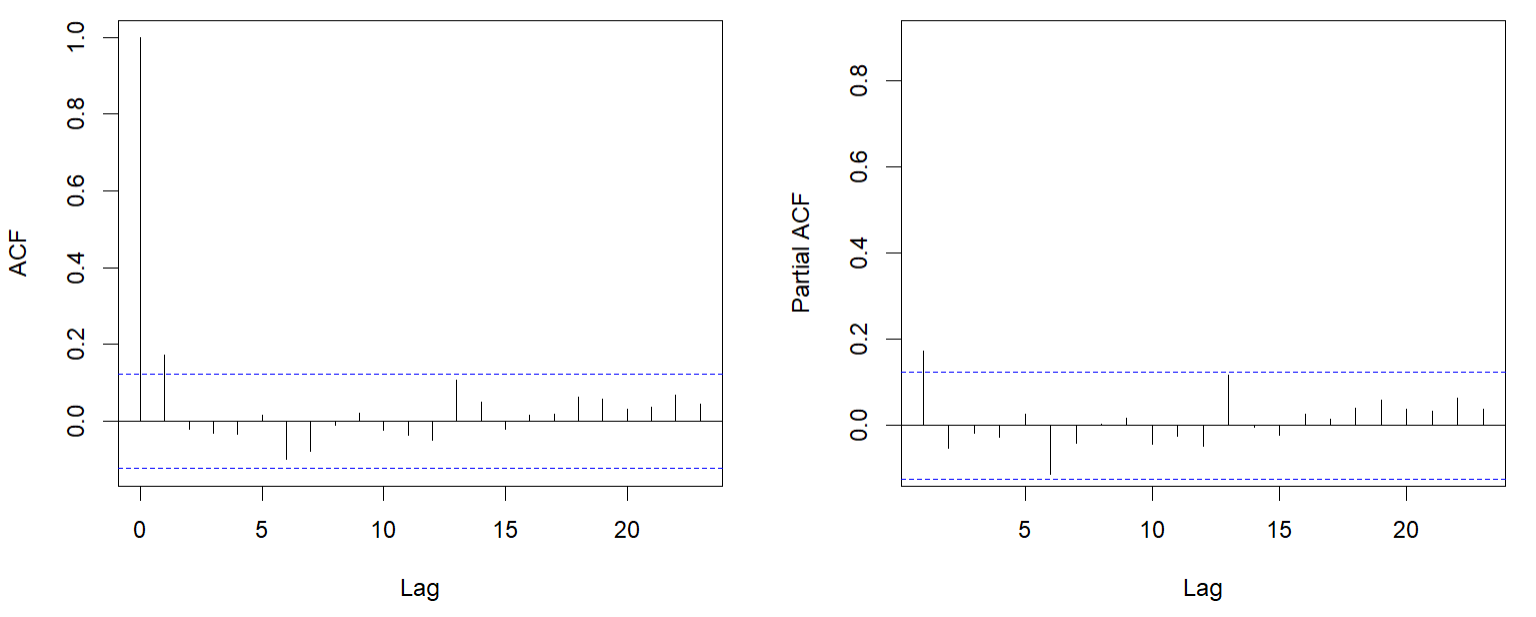
\includegraphics[width=0.9\textwidth]{acf_pacf.png}
    \caption{ACF AND PACF PLOTS}
    \label{fig:label5}
\end{figure}
\newpage

\subsection{Finding p and q using AIC Criteria:}
\[
\text{For ARMA}(p, q) \text{ model selection using AIC:}
\]
\[
\text{AIC} = -2 \log(L) + 2(p+q) \quad \text{, where } L \text{ is the likelihood of the model.}
\]
\[
\text{Choose values of } p \text{ and } q \text{ that minimize the AIC.}
\]




\begin{table}[h]
\centering
\begin{tabular}{|c|c|c|c|c|c|}
\hline
 & $q=0$ & $q=1$ & $q=2$ & $q=3$ & $q=4$ \\
\hline
$p=0$ & -456.99& \textbf{-461.55}& -459.78& -457.78& -456.04\\
\hline
$p=1$ & -461.00& -459.81& -457.78& -455.78& -456.44\\
\hline
$p=2$ & -459.77& -457.77& -457.82& -456.13& -454.39\\
\hline
$p=3$ & -457.77& -455.77& -456.29& -454.35& -452.59\\
\hline
$p=4$ & -455.77& -456.15& -454.34& -458.30& -452.97\\
\hline
\end{tabular}
\caption{AIC values for different combinations of $p$ and $q$. \\Highlighted: \textbf{-461.55}}
\textbf{p = 0 and q = 1}
\end{table}

Thus the final model is \textbf{ARIMA(0,1,1)}.
\begin{figure}[h]
    \centering
    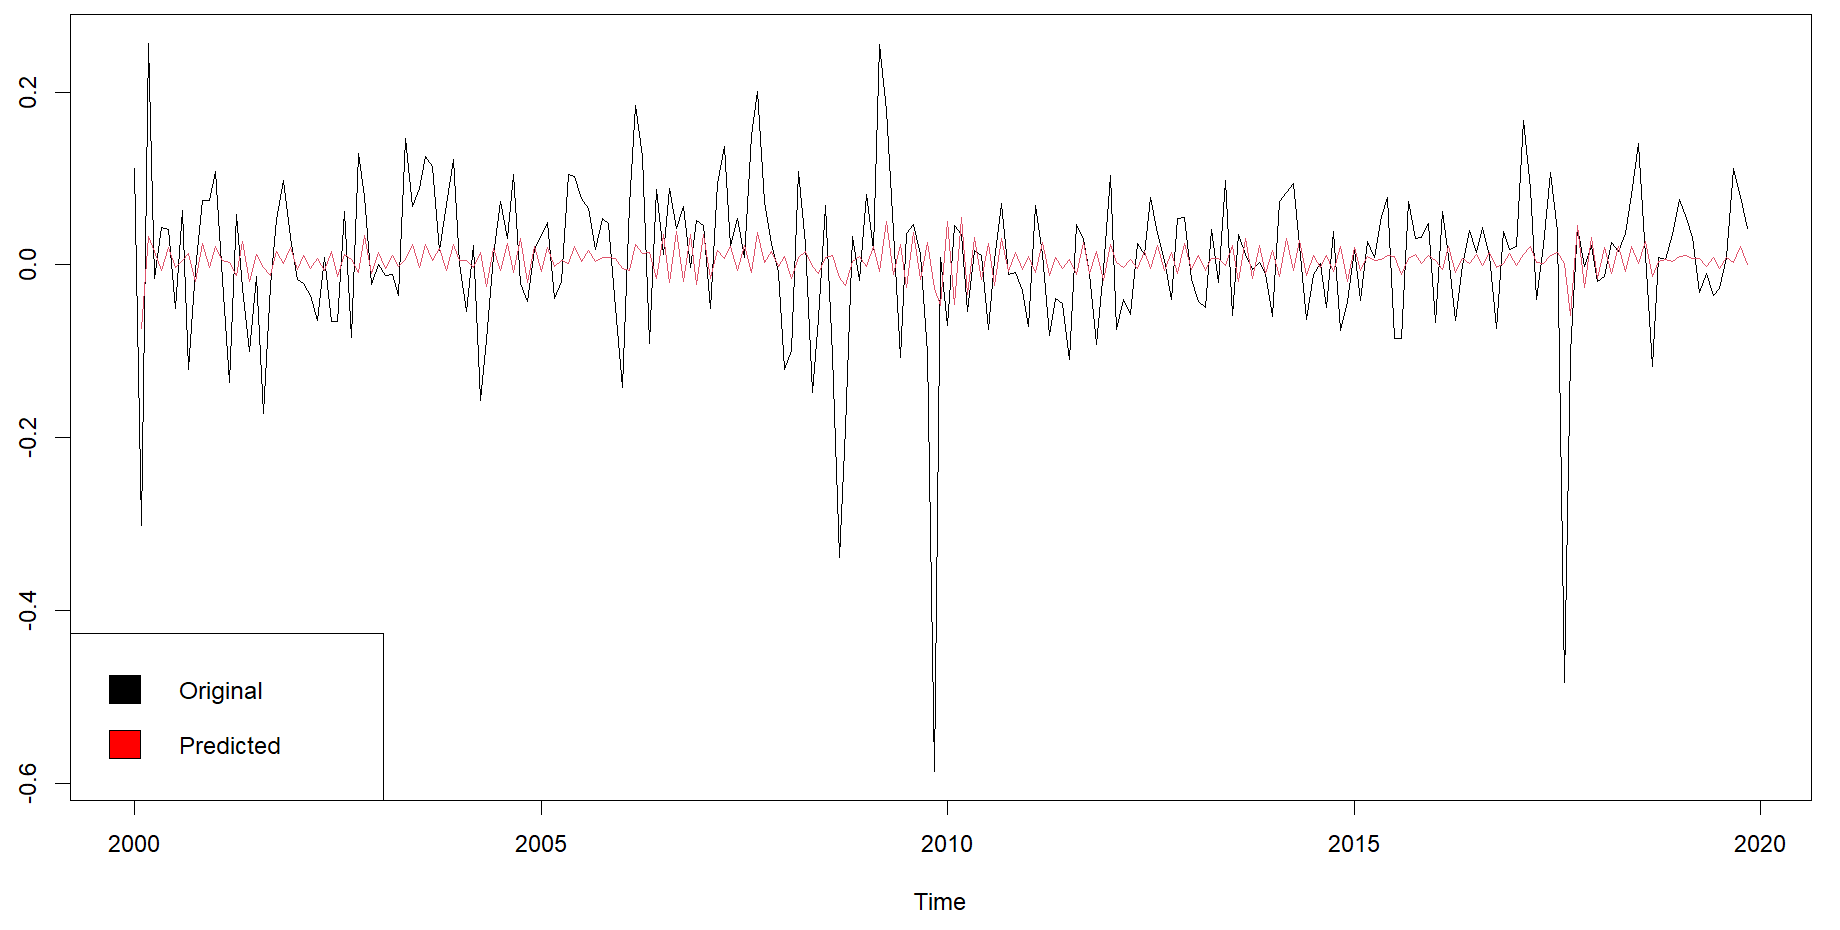
\includegraphics[width=0.9\textwidth]{Actual_vs_Predicted.png}
    \caption{Predicted vs Actual Detrended data}
    \label{fig:label6}
\end{figure}
\newpage

\section{Residual Analysis}{
\begin{figure}[h]
    \centering
    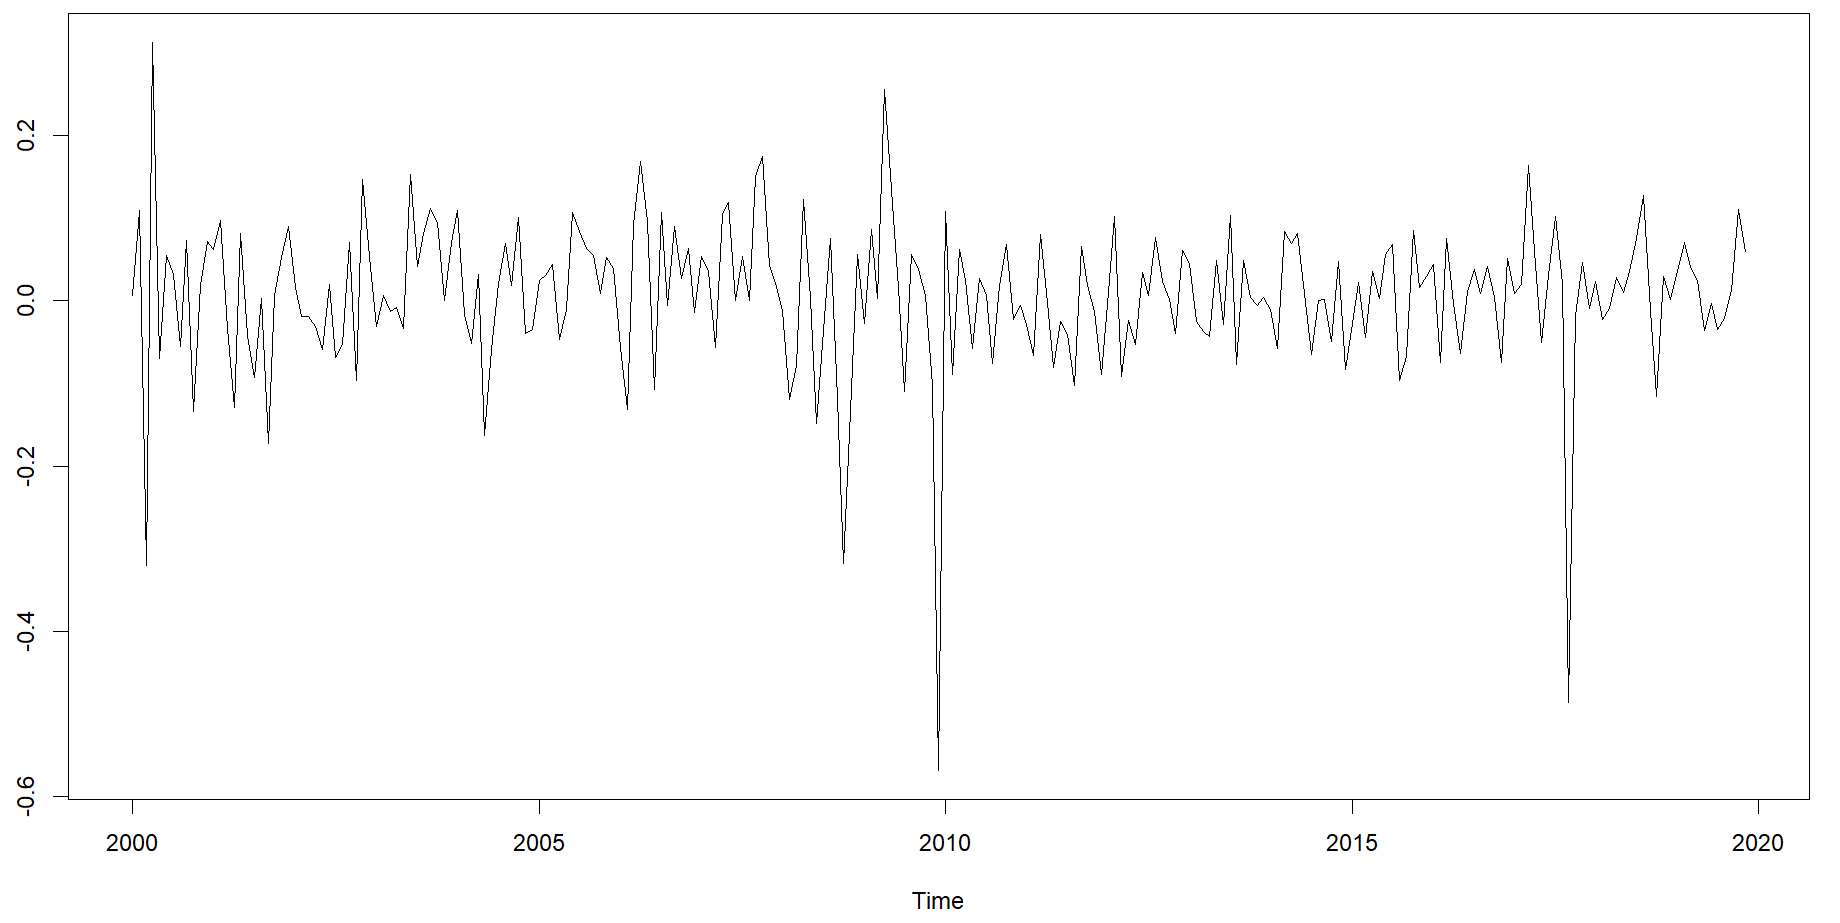
\includegraphics[width=0.9\textwidth]{Residuals.png}
    \caption{Plot of Residuals}
    \label{fig:label7}
\end{figure}
}

\begin{figure}[h]
    \centering
    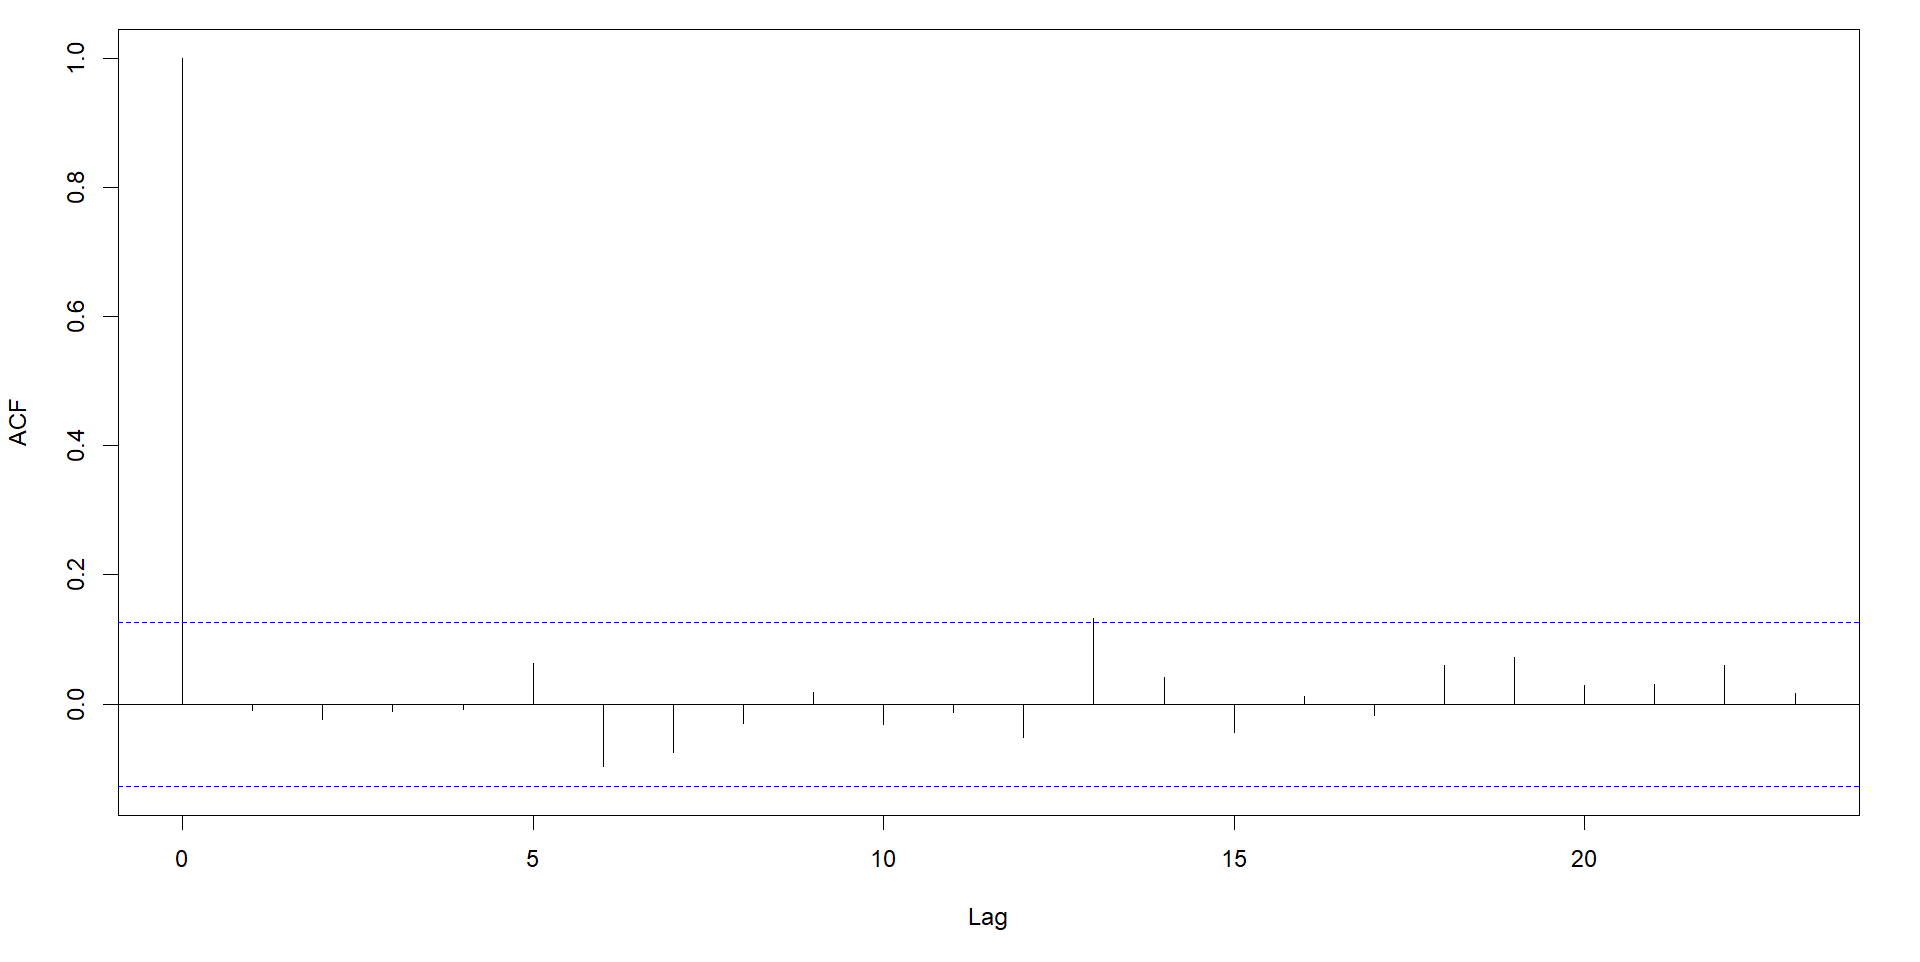
\includegraphics[width=0.9\textwidth]{acf_residuals.png}
    \caption{ACF of Residuals}
    \label{fig:label8}
\end{figure}

\begin{figure}[h]
    \centering
    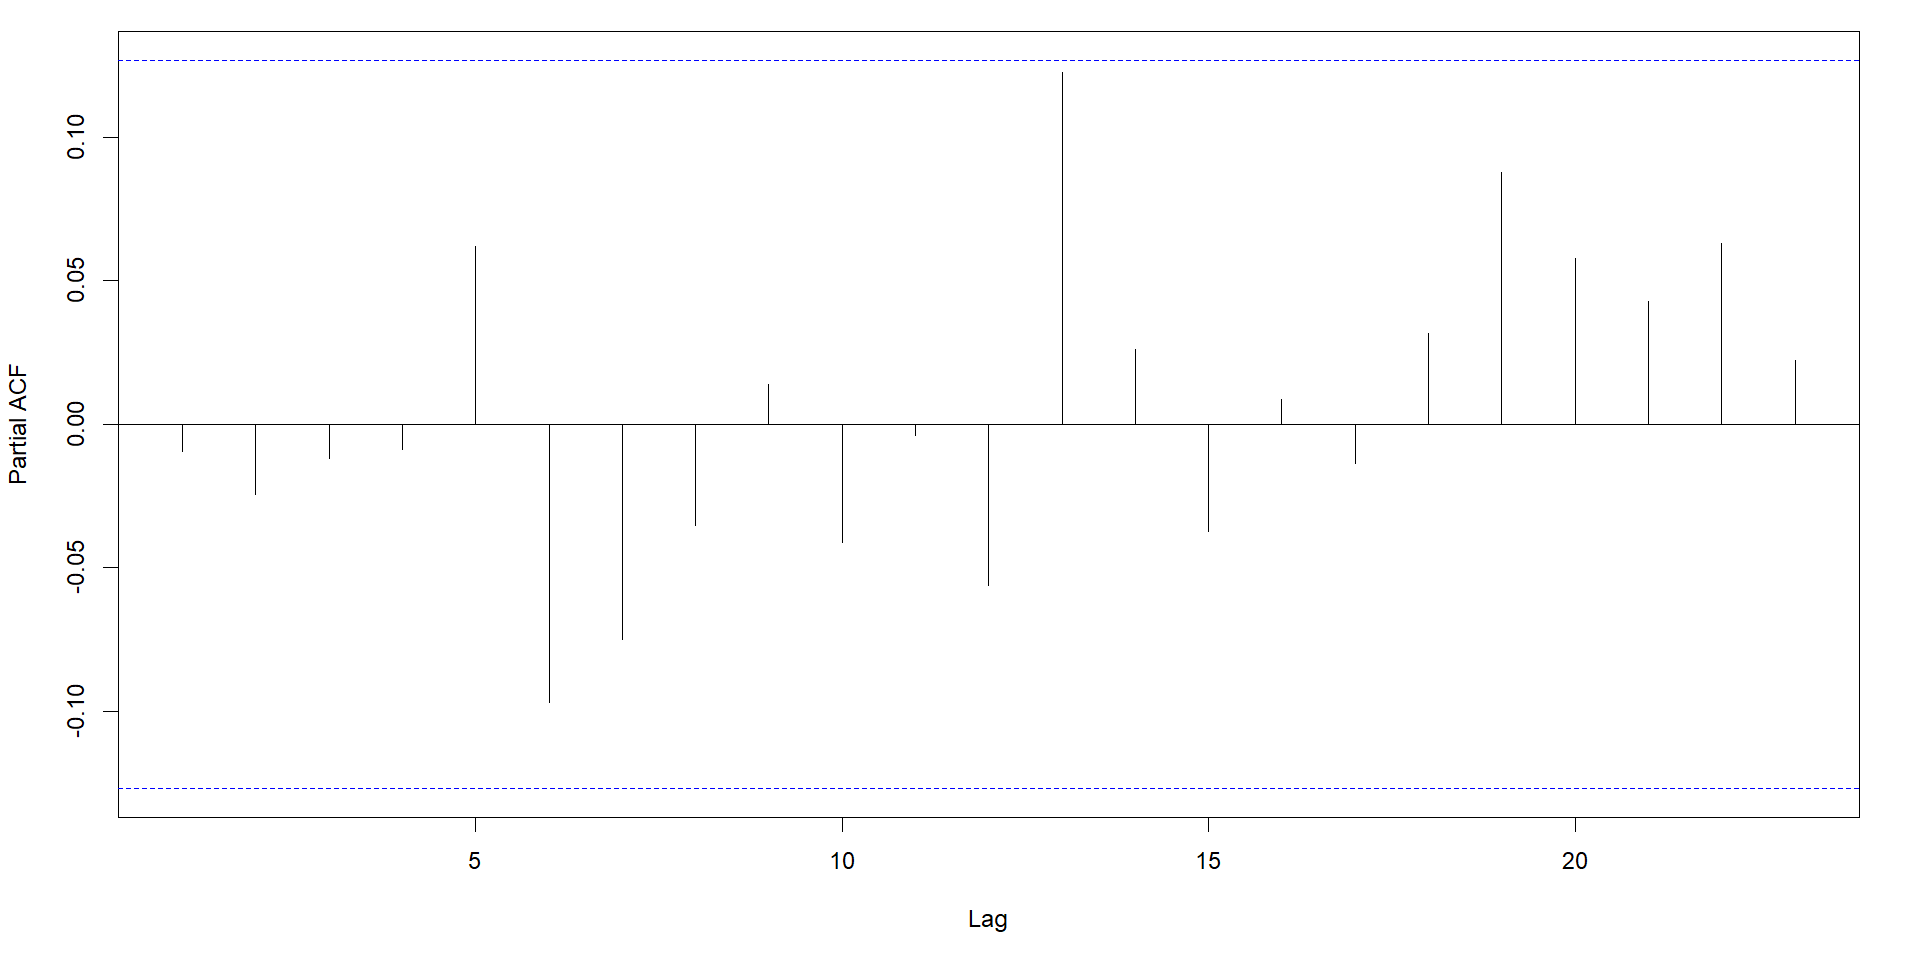
\includegraphics[width=0.9\textwidth]{pacf_residuals.png}
    \caption{PACF of Residuals}
    \vspace{1\baselineskip}
    \parbox{\linewidth}{According to ACF and PACF plots of the residuals we get to know it is a White Noise Process i.e. it means they are uncorrelated,
    but in the main plot we can see that the residuals are scaled, therefore before making the QQ plot we'll normalize them first}
    \label{fig:label9}
\end{figure}


\begin{figure}[h]
    \centering
    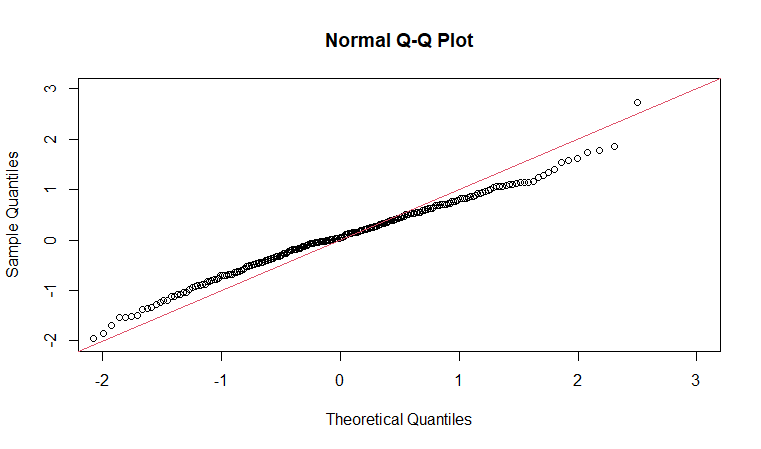
\includegraphics[width=0.9\textwidth]{qq_residuals.png}
    \caption{QQ Plot of Residuals}
    \label{fig:label10}
\end{figure}

\begin{figure}[h]
    \centering
    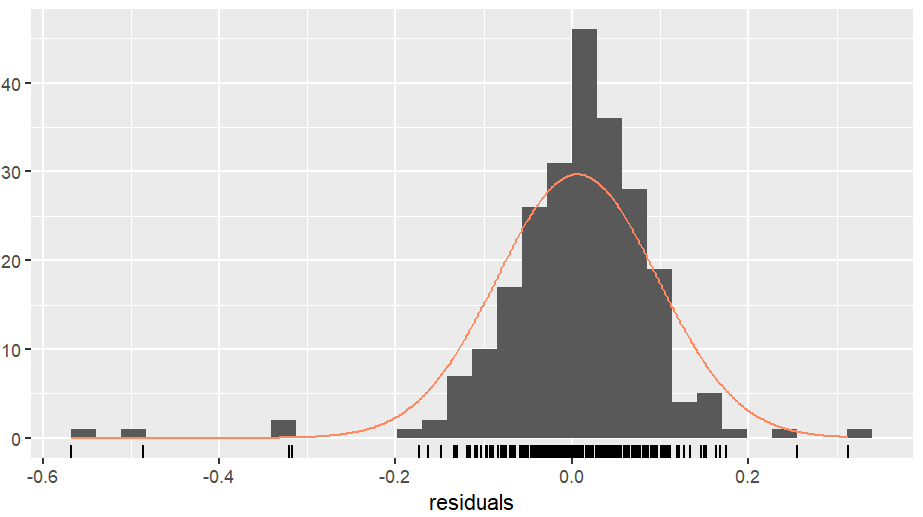
\includegraphics[width=0.9\textwidth]{hist_residuals.png}
    \caption{Histogram of Residuals}
    \vspace{1\baselineskip}
    \parbox{\linewidth}
    
    {\textbf{Conclusion:} We see that the residuals follow nomal distribution. \\ Thus we can say that the assumptions of the residuals are fulfilled.}
    
    \label{fig:label11}
\end{figure}

\begin{figure}[h]
    \centering
    \parbox{\linewidth}{\textbf{Forecasting values}}
    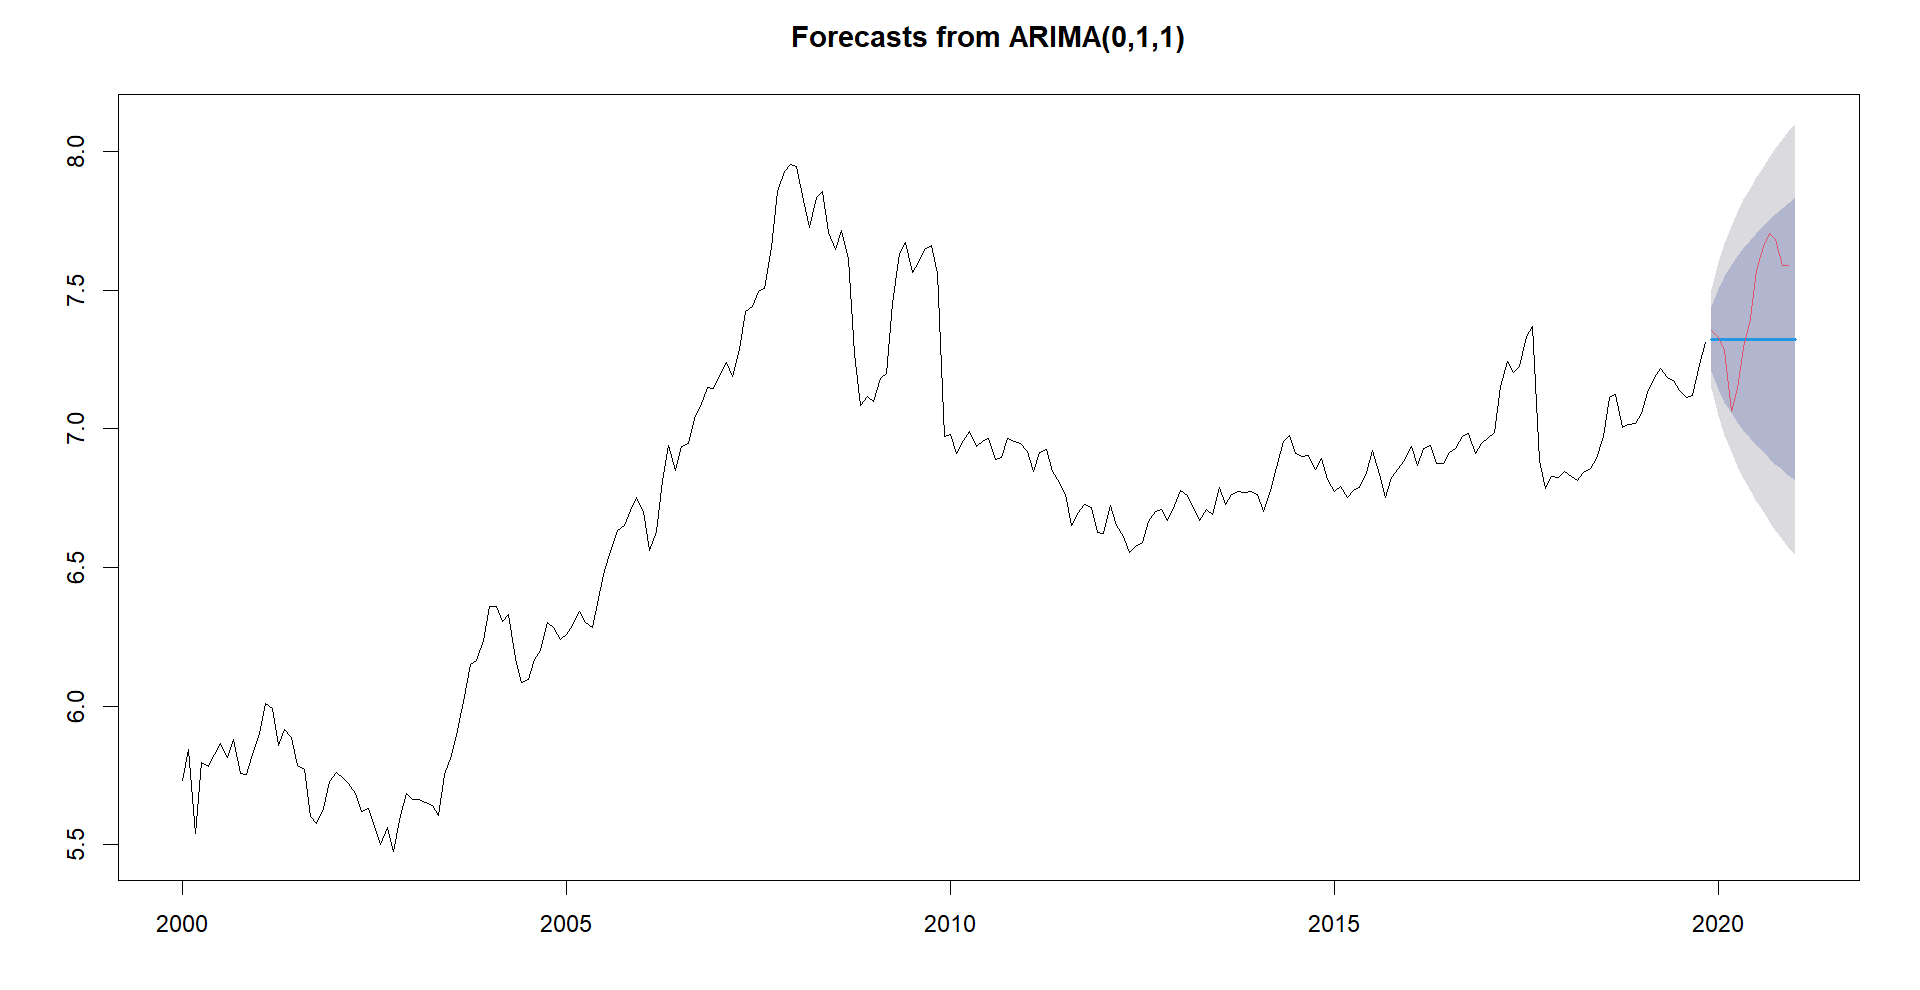
\includegraphics[width=0.9\textwidth]{Forecast.png}
    \caption{\textbf{Forecasting }}
    \vspace{1\baselineskip}
    \parbox{\linewidth}
    
    We see that the original values lies within our predicted range.
    \label{fig:label12}
\end{figure}
\end{document}
